\documentclass{article}

\usepackage{graphicx}
\usepackage{amsmath}
\usepackage{ctex}
\usepackage{url}

\usepackage{xcolor}
\usepackage{tikz}
\usetikzlibrary{arrows,shapes,chains}

\title{Mandelbrot-set和Julia-set}
\author{罗俊勋\\数学与应用数学\\3210101613}
\begin{document}
\maketitle
    % 摘要
    \begin{abstract}
        探讨Mandelbrot-Set和Julia-Set之间的关系,并使用Python实现set可视化
    \end{abstract}

    \paragraph{1.Julia和Mandelbrot简介}:\par
    Julia集是一个在复平面上形成分形的点的集合,它由法国数学家Gaston Julia最早发现。\cite{first}
    Julia集合可以由下式进行反复迭代得到:$f(x) = z^2 + c$
    , 其中z是复平面某一点,c是一个复常数。
    把这个公式反复迭代,最终会得到一个复数C,然后根据C的模长的大小,把这个点映射成不同的颜色.(这里用到的是python中imshow函数)
    漂亮的Julia集分形就出来了.
    每取一个不同的 c ,我们都能得到一个不同的 Julia 集,这些 Julia 集长相各异,稍微更改c的数值,就会对Julia集产生很大的影响,这些集合
    各有各的美丽.在 Julia 集相关领域中,有一个非常漂亮而且非常重要的定理叫做 $fundamental dichotomy theorem$ ,
    这个定理告诉我们,一个 Julia 集要么是完全连通的,任意两点间都有一条通路;要么是完全不连通的,整个图形全是一个个孤立的点
    随着常数 c 的变化,对应的 Julia 集也会连续地发生变化。想要探究的是,哪些 c 值会让对应的 Julia 集形成一个连通的区域?
    在研究 Julia 集时,通常假设 c 的模总是小于 2 的,因此,对任意一个满足 |z| > 2 的复数 z ,都有 $|z^2| = {|z|}^2 > 2·|z| $,
    也就是说,对这样的 z 进行平方后,它的模至少都会变成原来的两倍。即使常数 c 的方向和 z2 的方向完全相反,也不足以把 z2 的模抵消到原来的水平。
    因此,在迭代运算过程中,一旦某一步结果的模大于 2 了,可以断定它必将发散到无穷。因此,我们有了 Julia 集合的另一个定义。
     $z$ 到 $z^2 + c$ 对应的 Julia 集,就是无限迭代下去后模仍然不超过 2 的点。于是,我们给出Julia集的另外一个定义
     我们可以从复平面上模不超过 2 的所有点,也就是以原点为中心半径为 2 的圆盘出发,看看哪些点的平方加 c 后会落在这个圆盘内,
     进而考察哪些点平方加 c 再平方加 c 后将会落在这个圆盘内,如此反向迭代,不断找出原象,反推出符合要求的点集(Mandelbrot)。
     \cite{second}



     \paragraph{算法流程}
     \section{Julia集合的绘制流程图}


\begin{tikzpicture}[node distance=10pt]
  \node[draw, rounded corners]                        (start) 
  {$Z_{n+1} = z_{n}^2 + c$};
  \node[draw, below=of start]                         (step 1)
  {输入常数c和输入最高迭代次数n};
  \node[draw, below=of step 1]                        (step 2)
  {对一个复平面的点};
  \node[draw, diamond, aspect=3, below=of step 2]     (choice)
  {for z in $Z_n$};
  \node[draw, below=40pt of choice]  (step 3)
  {迭代下一个点};
  \node[draw, right=40pt of choice]  (step 4)
  {在集合中};
  \node[draw, left=40pt of choice]  (step 5)
  {不在集合中};
  
  \draw[->] (start)  -- (step 1);
  \draw[->] (step 1) -- (step 2);
  \draw[->] (step 2) -- (choice);
  \draw[->] (choice) -- node[left]  {}
  (step 3);
  \draw[->] (choice) -- node[above] {$|z| \geq 2$}
  (step 4);
  \draw[->] (choice) -- node[above] {$|z| < 2$}
  (step 5);
\end{tikzpicture}
     

     \paragraph{计算Mandelbrot}:\par
     为了判断 z → z2 + c 的 Julia 集是否连通,我们只需要测试一下,看对初始值 0 迭代无穷多次,所得的模是否会趋于无穷大。
     我们自然希望知道,能够使 Julia 集连通的常数值 c 在复平面上组成了一个什么样的图形。为此,我们只需要固定初始值为 0 .
     把复平面上不同的点当作 c ,画出迭代过程中模的发散速度,和最开始制作 Julia 集一样,我们用不同的颜色来表示不同的发散速度:
    运行Mandelbrot-set.py文件,得到其图片:
    这本身竟然又是一个漂亮的分形图形!\par 
    \begin{figure}[h]
        \centering
        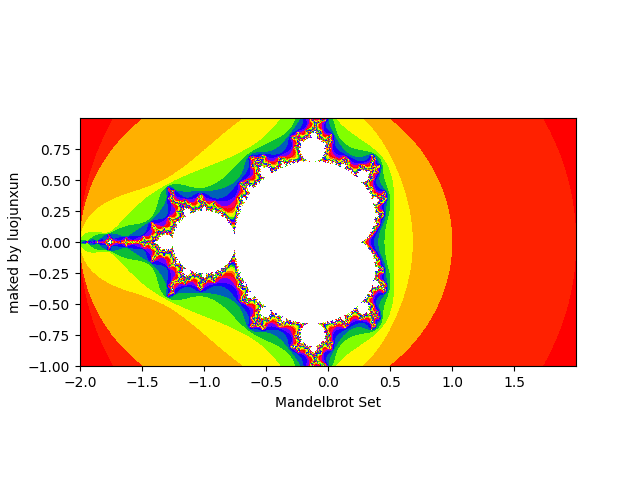
\includegraphics[scale = 0.8]{Mandelbrot-set.png}
    \end{figure}
    
    \paragraph{计算不同c下的Julia集合}:\par 
    在程序Julia-Set.py中
    分别取$c =-0.8+0.156i,c = 0.11+0.66i$得到两张Julia的分形图:图1和图2 (见下页)

    \begin{figure}[htbp]
        \centering
        \begin{minipage}[t]{0.48\textwidth}
        \centering
        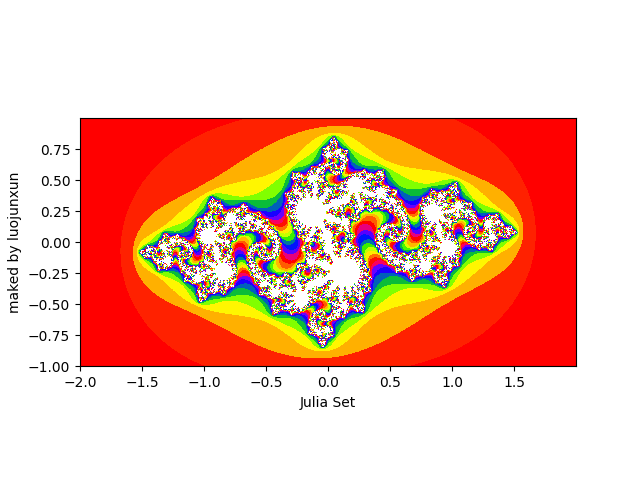
\includegraphics[width=6cm]{julia with c = (-0.8+0.156j).png}
        \caption{-0.8+0.156i}
        \end{minipage}
        \begin{minipage}[t]{0.48\textwidth}
        \centering
        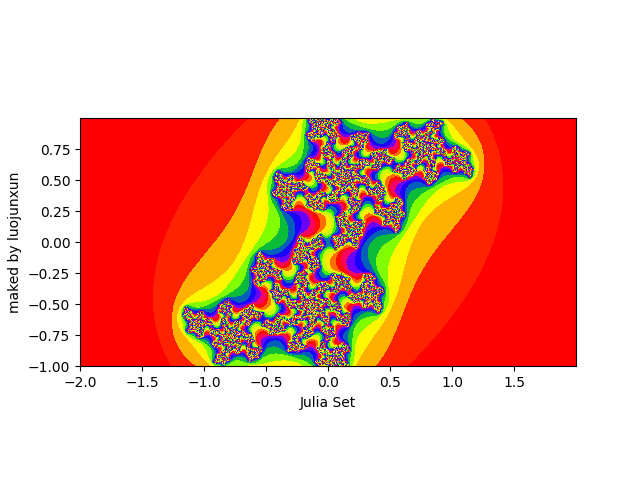
\includegraphics[width=6cm]{julia with c = (0.11+0.66j).png}
        \caption{0.11+0.66i}
        \end{minipage}
    \end{figure}
    \par
    再取$c = 0.188+0.78603i , n = 5$得到:Julia Set图(见下页)
    \begin{figure}[h]
        \centering
        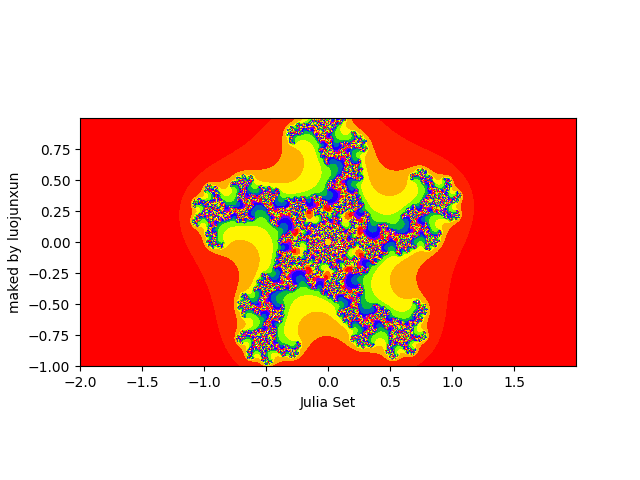
\includegraphics[scale = 0.6]{julia with c = (0.188+0.78603j).png}
    
    \end{figure}




    

    \paragraph{小结}:\par 
    让我们总结一下 Julia 集和 Mandelbrot 集的关系。在迭代过程 z → z2 + c 中,
    我们有四个参数: z 的初始值的实部、虚部,以及 c 的实部、虚部。 Julia 集就是给定 c 的实部
    、虚部后所得的结果,而 Mandelbrot 集则是限定 z 的实部和虚部均为 0 后的结果
    事实上,如果把所有不同的 Julia 集重合起来,我们将会得到一个四维图形,它的其中两个维度是不同的初始值
     z 构成的复平面,另外两个维度则是不同的常数 c 构成的复平面。这个四维空间就包含了所有不同的初始值在所有不同的常数
      c 之下迭代的发散情况。而 Mandelbrot 集,则是这个四维图形在 c = 0 处的一个切片,并且是最具有概括力的一个切片。
    \cite{second}




\bibliographystyle{plain}
\bibliography{ref}

\end{document}